For us to create a system that can implement the fingerprinting technique in a suitable way, we decided to develop a mobile application.
The benefit of using a mobile application rests on the fact that typical mobile devices already have the capability to interact and collect data from with Bluetooth devices, such as Bluetooh beacons.
This allowed us the integrate the process of collecting the data, doing classification with kNN and applying the resulting kNN model to conduct experiments within the same system.

A primary function of the application is to collect data from the aforementioned beacons. 
As illustrated in figure \ref{fig:ScanAdvertisement}, when the device is running, it will scan for advertisement packets projected by the Bluetooth beacons. 

\begin{figure}[H]
    \centering
    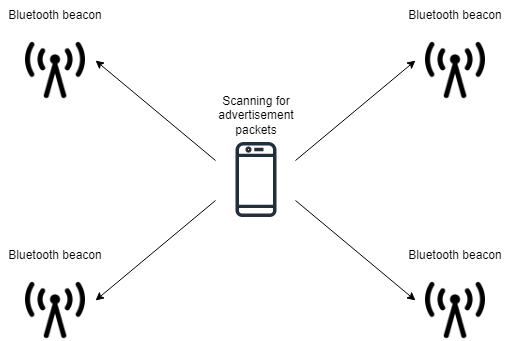
\includegraphics[width=0.8\textwidth]{images/ScanningForAdvertisement.drawio.png}
    \caption{}
    \label{fig:ScanAdvertisement}
\end{figure}

These packets contain information such as an identifier for the specific Bluetooth beacon along with RSSI data.
This information can then be collected 

%How it works with beacons
% which beacons

% Bridge between main report and implementation
% summarize that we have decided on using fingerprinting
% 
% We have found out that we need presence
% we have developed an app 

